\documentclass{article}
\usepackage{amsmath, graphicx}

\begin{document}
\title{PCA}
\author{}
\date{}
\maketitle

\section{Introduction}

PCA stands for principal components analysis and is a useful and commonly used data analysis technique in statistics, machine learning, and computer vision.  Let us start with an example involving students where a portion of the data for four students is shown in Table~\ref{tab:students}.  A scatter plot of this data (after subtracting the mean) for one hundred students is shown in Figure~\ref{fig:students}.  Note how the main direction of variation appears to be along the diagonal---this principal component of variation is exactly what is found by PCA.

\begin{table}
\centering
\begin{tabular}{rcc}
Student & Physics & Statistics \\
\hline
1 & 52.58 & 50.38 \\
2 & 66.47 & 71.68 \\
3 & 53.11 & 62.05 \\
4 & 68.28 & 41.83 \\
\end{tabular}
\caption{Each row is a student and the columns show test scores in physics and statistics.}
\label{tab:students}
\end{table}

\begin{figure}
\centering
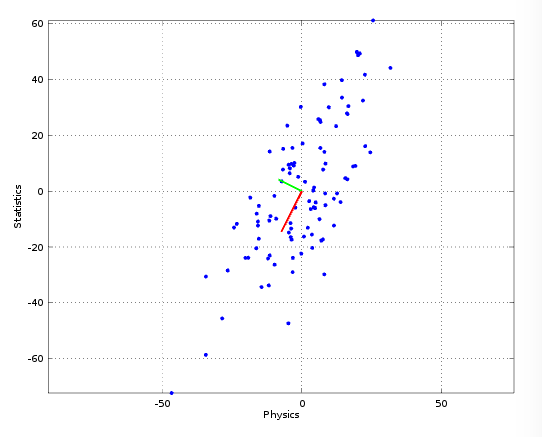
\includegraphics[width=3in]{physicsStatistics.png}
\caption{Scatter plot of physics and statistics test scores.  The red/green line segment is the first/second principal component.}
\label{fig:students}
\end{figure}

\section{Derivation}

One way to derive PCA is to formulate it as an optimization problem where the goal is to find the direction of maximum variance.  The direction can be represented as a unit norm vector $w$ where $\left\Vert w \right\Vert = 1$.  The data projected onto $w$ is $y_i = w'x_i$.  Assuming the data is zero mean, then the variance can be written out as,
\begin{align}
v &= \frac{1}{n} \sum_{i=1}^n y_i^2 \\
  &= \frac{1}{n} \sum_{i=1}^n (w' x_i)(w' x_i) \\
  &= \frac{1}{n} \sum_{i=1}^n (w' x_i)(x_i' w) \\
  &= w' \left(\frac{1}{n} \sum_{i=1}^n x_i x_i'\right) w \\
  &= w' C w,
\end{align}
where $C$ is the covariance matrix.  So the optimization problem is as follows:
\begin{equation}
\max_w \quad w' C w \quad \text{such that} \quad  w'w = 1.
\end{equation}
The above problem can be solved with Lagrange multipliers:
\begin{align}
L &=  w' C w + \lambda (w'w - 1) \\
\frac{\partial L}{\partial w} &= 2Cw - w\lambda w = 0 \\
Cw &= \lambda w.
\end{align}
The last line in the derivation above shows that $w$ is an eigenvector of the $C$, with eigenvalue $\lambda$.  By substitution, we can compute the variance as,
\begin{equation}
v = w' C w = w' \lambda w = \lambda,
\end{equation}
which means that we should choose the eigenvector $w_1$ with largest eigenvalue $\lambda_1$.

\section{Example}

The red line segment in scatter plot of Figure~\ref{fig:students} shows the principal direction $w_1$ for the student data, which matches the intuitive diagonal direction.  The student data was actually generated according to the following model:
\begin{align}
p_i &= 50 + 10 m_i + \epsilon_i \\
s_i &= 25 + 20 m_i + \nu_i,
\end{align}
where $m_i$ is the years of study in math for student $i$ and $p_i$ and $s_i$ are the physics and statistics scores and $\epsilon_i$ and $\nu_i$ is noise.  The corresponding full data for the four example students is shown in Table~\ref{tab:studentsFull}.  The model uses a linear model between math study and test score.  So the underlying factor explaining the test scores is actually years of study in math.  PCA exactly determines these types of linear correlations.  The PCA features are the data projected onto the principal component, namely $f_i = w_1' x_i$.  From Figure~\ref{fig:mathFeature} we can see that this feature is highly correlated with the years of study in math (the correlation coefficient is 0.92).  So PCA has essentially discovered the underlying math experience explanation for the correlation between the physics and statistics test scores.

\begin{table}
\centering
\begin{tabular}{rccc}
Student & Math & Physics & Statistics \\
\hline
1 & 0.75 & 52.58 & 50.38 \\
2 & 2.08 & 66.47 & 71.68 \\
3 & 0.83 & 53.11 & 62.05 \\
4 & 1.08 & 68.28 & 41.83 \\
\end{tabular}
\caption{Each row is a student and the columns show years of study in math and test scores in physics and statistics.}
\label{tab:studentsFull}
\end{table}

\begin{figure}
\centering
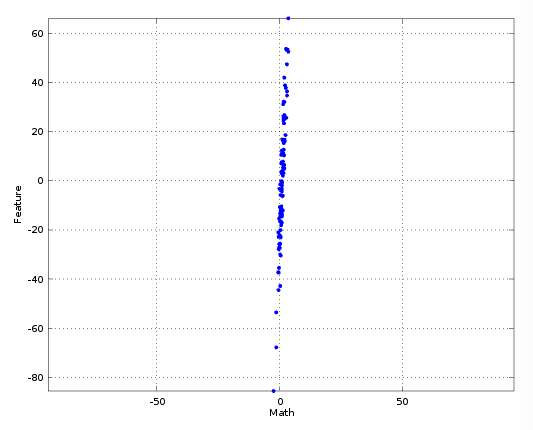
\includegraphics[width=4in]{mathFeature.png}
\caption{Scatter plot of math study and principal component feature.  The correlation coefficient is 0.92.}
\label{fig:mathFeature}
\end{figure}

\section{Geometric Example}

From the scatter plot shown in Figure~\ref{fig:students}, one can see that there is a geometric interpretation of PCA, namely that it finds the axis of least inertia of the shape approximated by the points.  In computer vision, PCA is often applied to a point set from the pixel locations describing a shape to find the orientation of the shape.  An example of this is shown in Figure~\ref{fig:snoopy}, where the black pixel locations are the points input to PCA and the red line segment is the principal component or axis of least inertia, which can be used to represent the orientation of Snoopy in the image.

\begin{figure}
\centering

\includegraphics[width=2in]{Snoopy.png} 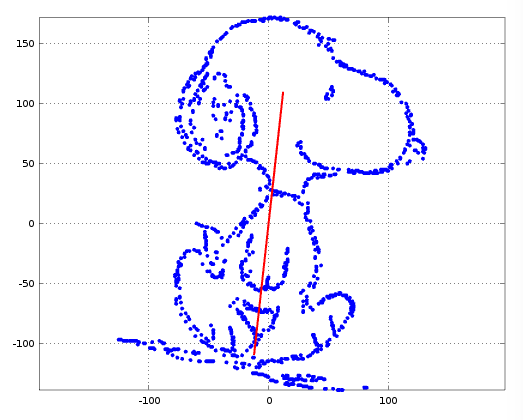
\includegraphics[width=2.5in]{snoopyPCA.png}
\caption{Left: input image of Snoopy.  Right: PCA output of blue points.}
\label{fig:snoopy}
\end{figure}

\end{document}
